%% GENERATED by paper/scripts/make_paper_assets.py -- do not edit by hand.
%% source: eval/generations/ag1-v4-360-single.jsonl (regraded)
\begin{figure}[t]
\centering
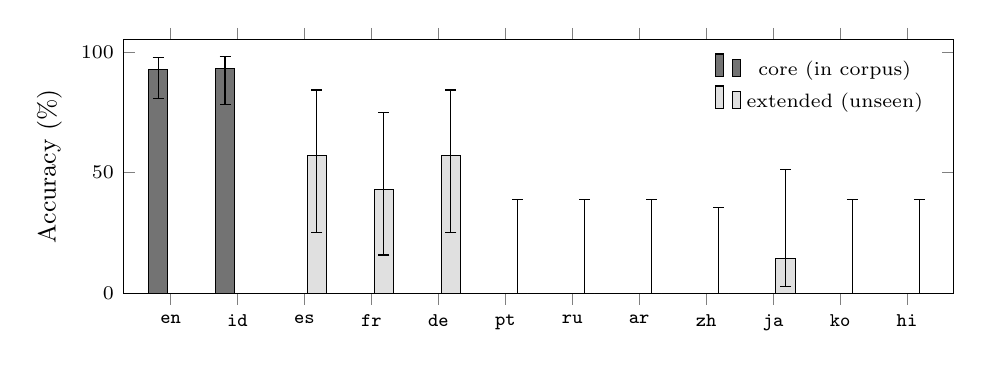
\begin{tikzpicture}
\begin{axis}[
  width=\columnwidth, height=4.8cm,
  ybar, ymin=0, ymax=105,
  ylabel={Accuracy (\%)},
  xtick={0,1,2,3,4,5,6,7,8,9,10,11}, xticklabels={en,id,es,fr,de,pt,ru,ar,zh,ja,ko,hi},
  x tick label style={font=\scriptsize\ttfamily}, y tick label style={font=\scriptsize},
  label style={font=\small},
  bar width=7pt, enlarge x limits={abs=0.7},
  error bars/y dir=both, error bars/y explicit,
  legend style={font=\scriptsize, at={(0.98,0.97)}, anchor=north east, draw=none,
    fill=none, legend columns=1},
]
\addplot[fill=black!55, draw=black] coordinates {(0,92.6829268292683) += (0,4.817073170731703) -= (0,12.082926829268288) (1,93.10344827586206) += (0,4.99655172413793) -= (0,15.103448275862064)};
\addlegendentry{core (in corpus)}
\addplot[fill=black!12, draw=black] coordinates {(2,57.14285714285714) += (0,27.057142857142864) -= (0,32.14285714285714) (3,42.857142857142854) += (0,32.142857142857146) -= (0,27.057142857142853) (4,57.14285714285714) += (0,27.057142857142864) -= (0,32.14285714285714) (5,0.0) += (0,39.0) -= (0,0.0) (6,0.0) += (0,39.0) -= (0,0.0) (7,0.0) += (0,39.0) -= (0,0.0) (8,0.0) += (0,35.4) -= (0,0.0) (9,14.285714285714285) += (0,37.01428571428572) -= (0,11.685714285714285) (10,0.0) += (0,39.0) -= (0,0.0) (11,0.0) += (0,39.0) -= (0,0.0)};
\addlegendentry{extended (unseen)}
\end{axis}
\end{tikzpicture}
\caption{Becussy One per language, Wilson 95\% intervals. The two core languages are the
only ones in the training corpus. Transfer reaches Spanish, German, French and a trace of
Japanese, then stops dead: Portuguese, Russian, Arabic, Chinese, Korean and Hindi are
exactly zero. Extended $n$ is 6--7 per language, so the intervals are wide by
construction.}
\label{fig:perlang}
\end{figure}
